\section{Langkah-Langkah Percobaan}
\subsection{Crimping}
\subsubsection{Mempersipakan Alat dan Bahan}
Sebelum memulai praktikum, praktikan memersiapkan beberapa alat dan bahan yang diperlukan. Alat dan bahan telah disediakan dimana perwakilan dari kelompok praktikan mengambil 2 buah kabel UTP, 4 buah RJ45, LAN Tester, dan, satu set perlatan crimping yang  meliputi tang crimping, pemotong kabel, dan tools sejenis. 

\subsubsection{Mempersiapkan Kabel LAN}
Setiap praktikan bertanggung jawab untuk satu ujung kabel UTP. Praktikan pertama-tama mengupas pembungkus luar kabel dengan perkiraan panjang satu ruas jari kemudian memisahkan pilinan kabel-kabel yang lebih kecil. Kabel-kabel kecil tersebut lalu disusun rapi dengan urutan T568B. Pada kasus penulis, susunan kabel tidak rata, sehingga kabel dipangkas sedikit menggunakan alat. 

\subsubsection{Melakukan Crimping}
Susunan kabel yang sudah rapi dan benar dimasukkan ke RJ45. Praktikan perlu memperhatikan jangan sampai pemasangan RJ45 terbalik antar atas dan bawahnya. Ujung kabel yang sudah terpasang RJ45 dimasukkan ke dalam mesin crimping dan ditekan hingga terdengan bunyi "krek". Kabel UTP selesai di-crimping.

\subsection{Routing}
\subsubsection{Mempersipakan Alat dan Bahan}
Sebelum memulai percobaan kedua ini, praktikan memersiapkan beberapa alat dan bahan yang diperlukan. Alat dan bahan yang praktikan bawa sendiri diantaranya, laptop yang sudah terinstall Winbox, dan kabel UTP. Sedangkan alat dan bahan yang telah disediakan adalah 2 set router mikrotik. Pengambilan dilakukan oleh perwakilan kelompok.

\subsubsection{Merangkai Router dengan Laptop}
Pada router 1, interface ether 6 dihubungkan dengan laptop 1. Sedangkan interface ether 7 dihubungkan dengan interface ether 7 dari router ether 2. Pada router 2, interface ether 6 dihubungkan dengan laptop 2. 

\subsubsection{Routing Statis}
\begin{enumerate}
  \item Mengkonfigurasi alamat statis untuk semua interface\\
  Pada laptop 1, untuk mengkonfigurasi interface dari router 1, praktikan menggunakan aplikasi Winbox. Pada aplikasi winbox, praktikan login ke alamat default untuk mengakses konfigurasi router. Berdasarkan arahan dari modul, interface ether 6 yang terhubung ke laptop 1 diberi alamat 192.168.10.1/27 dan ether 7 yang terhubung ke router 2 diberi alamat 10.10.10.1/30. dengan cara yang sama menggunakan laptop 2, router 2 juga dikonfigurasi sedemikian hingga ether 6 memiliki alamat 10.10.10.2 dan ether 7 memiliki alamat 192.168.20.1/27. Praktikan juga memberikan alamat IP statis untuk laptop 1 dan 2 dengan mengeditnya melalui setting. Laptop 1 diberi alamat 192.168.10.2/27 dan laptop 2 diberi alamat 192.168.20.1/27.
  \item Menambahkan Routing Table \\
  Agar laptop 1 dan laptop 2 dapat berkomunikasi, diperlukan adanya routing. Praktikan membuat routing table untuk router 1 dan router 2 melalui menu IP > Routes. Karena subnet yang tidak terhubung langsung ke masing-masing router hanya 1, maka hanya perlu menambahkan 1 untuk masing-masing router. Untuk router 1, praktikan menambahkan 1 data routing dengan Dest Addres : 192.168.20.0/27 dan Gateway : 10.10.10.2. Sedangkan untuk router 2, praktikan menambahkan 1 data routing dengan Dest Addres : 192.168.10.0/27 dan Gateway : 10.10.10.1. 
  \item Mengkonfigurasi gateway laptop \\
  Seperti ketika mengkofigurasi alamat laptop, praktikan mengedit setting > Network \& Internet > Ethernet > IP Assignment dengan IP, subnet, dan gateway sesuai arahan modul. 
  \item Memeriksa Koneksi \\
  Untuk memeriksa apakah routing sudah berhasil, laptop akan melakukan ping ke setiap alamat interface. Uji ping yang dilakukan praktikan di laptop 1 ke interface ether 6 router 1 dan ke laptop 2 menghasilkan reply (artinya bisa terkoneksi). Kelompok praktikan sempat mengalami masalah karena ping tidak berhasil (tidak ada reply) karena kesalahan menulis gateway dan routing table.
\end{enumerate}

\subsubsection{Routing Dinamis}
\begin{enumerate}
  \item Konfigurasi router\\
  Untuk menghemat waktu, kelompok praktikan tidak melakukan reset pada router dan mengkonfigurasi interface dari awal.
  \item Memastikan Routing RIP Aktif\\
  Router mikrotik yang digunakan sudah merupakan versi terbaru, sehingga Routing PID Package sudah aktif secara default.
  \item Mengkonfigurasi DHCP Server\\
  Berbeda dengan routing statis, untuk routing dinamis, pengalamatan interface dilakukan dengan dinamis oleh DHCP server. Praktikan masuk ke menu IP > DHCP server untuk melakukan setup alokasi address pool untuk setiap interface. 
  \item Konfigurasi Routing Dinamis Menggunakan RIP
  Pertama-tama, praktikan menambahkan interface sesuai arahan modul. Setelah itu, praktikan memasukkan semua network address yang terhubung ke router. pada router 1 192.168.10.0/27 dan 10.10.10.0/30 Sedangkan pada router 2 192.168.20.0/27 dan 10.10.10.0/30. Selanjutnya, praktikan menambahkan gateway untuk neighbours network pada menu RIP > Neighbours
  \item Mengubah Konfigurasi Laptop
  Sebelunya pada routing dinamis, praktikan menetukan IP untuk laptop. Pad percobaan dinamis ini, praktikan mengubah kembali setting menjadi otomatis DHCP server.
  \item Uji Ping
  Untuk memastikan konfigurasi benar, praktikan melakukan ping ke interface router 1, intercafe router 2, dan ke laptop lainnya.
\end{enumerate}

\section{Analisis Hasil Percobaan}
Pada praktikum crimping, kelompok praktikan telah berhasil crimping 2 buah kabel dengan konfigurasi cross over. Kabel ini pun telah diuji dan dipakai untuk praktikum, baik routing dinamis maupun statis, dan bekerja dengan cukup baik. Berdasarkan teori, kabel scross over seharusnya hanya digunakan untuk komunikasi perangkat sejenis, namun dalam praktikum ini, praktikan menggunakannya untuk perangkat berbeda jenis, yaitu router dan laptop. Ternyata, untuk router moderen saat ini, telah dilengkapi dengan MDI.MDI-X sehingga dapat otomatis mengatur sinyal TX dan RS di port Ethernet. Dengan begitu, menggunakan kabel cross over atau straight through tidak menjadi masalah. \\
Pada praktikum routing statis, kelompok praktikan juga telah berhasil melakukan konfigurasi untuk semua perangkat dan melakukan komunikasi antar perangkat. Pada praktikum ini, praktikan menerapkan penggunaan subnet untuk mebagi network menjadi sub network yang lebih kecil, yaitu 3 subnet A (laptop 1), B (laptop 2), dan subnet antara router dengan ukuran yang disesuaikan dengan kebutuhan device nya. Ketika praktikum, kelompok sempat melakukan kesalahan dalam konfigurasi routing yang menyebabkan gagalnya komunikasi dengan laptop lannya meskipun komunikasi dengan interface router terhubung tetap berjalan baik. Hal ini sesuai dengan teori bahwa perangkat dalam satu subnet dapat berkomunikasi secara langsung, sedangkan komunikasi dengan perangkat dari subnet lain harus melalui routing. \\
Pada percobaan routing statis, kelompok praktikan berhasil melakukan konfigurasi dan komunikasi antar interface device. Praktikan melakukan konfigurasi DHCP untuk membuat perangkat endpoin menerima alamat secara acak dari pool.Didaptkan hasil, bawa pada laptop 1 berhasil mendapatkan ip 192.168.10.300. Sedangkan pada laptop dua mendapatkan 192.168.20.2.   Routing dinamis yang digunakan dalam praktikum ini adalah RIP. Konfigurasi RIP pada routing dinamis dan statis menggunakan RIP agak berbeda. Pada routing statis, praktikan harus memasukkan konfigurasi interface satu per satu. Sedangakan pada routing dinamis praktikan hanya perlu konfigurasi RIP interfaces untuk all ether untuk memungkinkan pertukaran informasi. namun, juga perlu melakukan setting network yang terhubung dan neighbors. Dengan konfigurasi ini, routing sudah dapat dialkukan tanpa membuat routing table secara manual.\\

\section{Hasil Tugas Modul}
\begin{enumerate}
  \item Berdasarkan tugas pendahuluan pada laporan sementara, berikut ini merupakan simulasi di cisco packet tracer \\
  	\begin{figure}[H] 
    \centering
    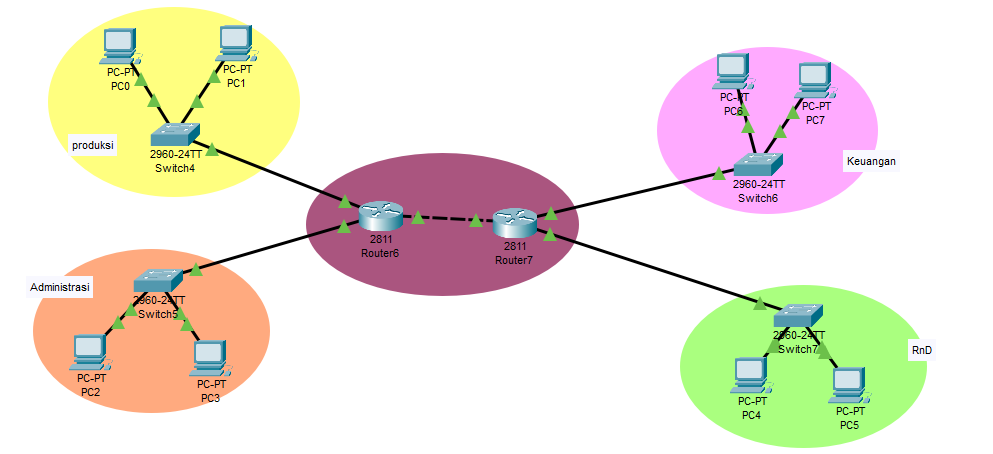
\includegraphics[width=0.5\textwidth]{P1/img/tupen3.png}
    \caption{Simulasi pada Cisco Packet Tracer}
    \label{fig: Simulasi pada Cisco Packet Tracer}
	\end{figure}
  Simulasi yang digunakan sebagaimana dapat dilihat di file \href{run:P1.pkt}{P1.pkt} [Lihat folder P1 > P1.pkt]
  \item 
  Selama praktikum, tantangan pertama  yang dihadapi adalah ketidakfamiliaran. Karena praktikan baru pertama kali melakukan crimping dan baru pertama kali juga melakukan konfigurasi untuk router mikrotik. Praktikan juga sempat bingung router mana dan interface mana yang harus memakai alamat.
\end{enumerate}

\section{Kesimpulan}
Kesimpulan berisi ringkasan dari hasil praktikum dan hal-hal penting yang didapatkan. Bagian ini menjawab tujuan praktikum, mencantumkan hasil yang sesuai atau tidak sesuai dengan teori, serta pembelajaran yang diperoleh oleh praktikan.\\
Berdasarkan praktikum yang telah dilakukan, praktikan telah berhasil menyelesaiakn praktikum dengan cukup sukses dengan hasil sesuai ekspektasi modul dan ekspektasi praktikan sendiri. Terdapat beberapa hal penting yang praktikan dapatkan selama praktikum ini. Pertama adalah penggunaan cble cross over dan straigh through yang kini sudah bisa \textit{interchangable}. Kedua, konfigurasi subnet yang sangat mempengaruhi pool dari host address nya. Ketiga, penggunaan subnet membatasi jaringan untuk berkomunikasi dengan perangkat dari jaringan lain. Keempat, pada routing dinami, routing table dibuat secara otomatis, dan masih banyak lagi. Setelah melakukan praktikum ini, praktikan merefleksikan dan lebih memahami bagaimana networking dan konfigurasi jaringan dapat dilakuakn.

\section{Lampiran}
\subsection{Dokumentasi saat praktikum}


\subsection{Hasil Challenge Modul}
Challenge pada praktikum ini adalah membuat mengembangkan konfigurasi dari praktikum dengan tambahan 2 switch (router yang dibuat menjadi switch) dan perubahan ukuran subnet menjadi untuk 100 perangkat dan 200 perangkat. \\
Kelompok praktikan berhasil menyelesaikan challenge. Praktikan memasukan konfigurasi subnet untuk laptop sebesar /24 untuk 200 perangkat dan /25 untuk 100 perangkat. Pada dua router tambahan, agar bisa berfungsi sebagai switch, praktikan menambahkan brige untuk semua interface dari router, tidak perlu melakuakn konfigurasi alamat dan routing.


